\section{Results}
\label{sec:results}

\subsection{Accuracy is below the trivial ceiling, and discrimination is at chance}
\label{sec:results-accuracy}

On the NIH clean cell, the majority-class ceiling over the seven pathology labels (all seven negative; \texttt{no\_finding} excluded) is \textbf{0.6579} of label slots. No model exceeds it by more than 1.0\,\pp{}; the best (InternVL3.5, 0.6674) is +0.95\,\pp{}, and Qwen2.5-VL (0.6578) is \emph{below} the ceiling. Clean AUROC is 0.50--0.63 for every model (Table~\ref{tab:clean}). An accuracy-first report would describe this table as ``0.54--0.67 accuracy''; the same table with a ceiling makes it ``no usable discrimination anywhere.'' The supervised replication of this claim is Section~\ref{sec:results-baseline}.

\begin{table}[t]
\centering
\small
\caption{Clean NIH performance vs.\ the always-negative ceiling over the seven pathology labels (\texttt{no\_finding} excluded; $n=1{,}506$ studies, 10,542 pathology slots). The ceiling is evaluated on each model's definite slots: 0.6579, except CheXagent at 0.6570 because only 18.9\% of its slots carry a definite status. Macro AUROC is over the seven pathology labels with a 95\% patient-cluster bootstrap interval (1,000 resamples; a missing probability is scored 0.0, matching script 75).}
\label{tab:clean}
\begin{tabular}{lrrrrr}
\toprule
Model & Pooled acc. & vs.\ ceiling & Macro AUROC [95\% CI] & Macro ECE & Positive recall \\
\midrule
InternVL3.5 & 0.6674 & $+1.0$\,\pp{} & 0.6066 [0.5949, 0.6191] & 0.247 & 0.4928 \\
MedGemma-1.5 & 0.6106 & $-4.7$\,\pp{} & 0.5852 [0.5748, 0.5952] & 0.234 & \textbf{0.6392} \\
MedGemma-4B & 0.5398 & $-11.8$\,\pp{} & 0.6270 [0.6138, 0.6394] & 0.207 & 0.5519 \\
Qwen3-VL & 0.5926 & $-6.5$\,\pp{} & 0.5455 [0.5350, 0.5568] & 0.348 & 0.1625 \\
Qwen2.5-VL & 0.6578 & $\mathbf{-0.01}$\,\pp{} & 0.5013 [0.5003, 0.5027] & 0.412 & 0.0039 \\
CheXagent & 0.0589 & $-59.8$\,\pp{} & 0.5001 [0.5000, 0.5002] & 0.310 & 0.0003 \\
\bottomrule
\end{tabular}
\end{table}

Macro ECE is reported as a descriptive reliability summary, not as a calibration claim: probabilities are verbalised inside the reply and exist only for definite slots, CheXagent has no probability channel at all, and no post-hoc calibration is applied. The AUROC column is therefore the only discrimination quantity in this table that is comparable across all six models.

\subsection{Degradation can raise recall by moving the operating point}
\label{sec:results-op}

Table~\ref{tab:op} reports severe-vs-clean changes at the pooled level. The operating-point cases are those with a high clean positive-prediction rate; models with a low baseline have no room to shift upward. This is a property of the \emph{measurement regime}, not a claim that degradation is harmless: precision falls in both InternVL3.5 rows ($-1.38$ and $-0.64$\,\pp{}), Qwen3-VL's precision rises slightly ($+0.19$\,\pp{}), and in all three cells the positive-prediction rate rises while false positives increase by 16\%, 8\%, and 20\%. The InternVL3.5 contrast increase is concentrated in pneumonia ($+98$) and consolidation ($+69$), 64.5\% of the 259 additional false positives, with none for pneumothorax (Table~\ref{tab:flip}). A patient-cluster bootstrap (1,000 resamples; \url{scripts/85_operating_point_ci.py}) gives $\Delta$recall $+4.69$ $[3.75,5.56]$, $+2.52$ $[1.46,3.63]$, and $+3.44$ $[2.37,4.69]$\,\pp{} for the three cells, and $\Delta$positive-prediction rate $+4.06$ $[3.44,4.64]$, $+2.09$ $[1.36,2.85]$, and $+2.51$ $[1.75,3.26]$; every interval excludes zero. The precision change excludes zero only for InternVL3.5 contrast ($-1.38$ $[-2.16,-0.63]$\,\pp{}); for the other two the interval includes zero. For the InternVL3.5 contrast cell, the case-level transitions (Appendix~\ref{app:risk}, Table~\ref{tab:flip}) show a broad reclassification rather than a targeted recovery of lost findings; the fixed-rule rerun below shows that the score distribution itself moves, so we label the pattern an operating-point shift, not a proven threshold change. A post-hoc fixed $0.5$ cut on the emitted probability reproduces the same change ($+4.80$ vs.\ $+4.69$\,\pp{} for contrast, $+2.47$ vs.\ $+2.52$\,\pp{} for brightness, $+3.36$ vs.\ $+3.44$\,\pp{} for Qwen3-VL; Appendix~\ref{app:risk}, Table~\ref{tab:fixedthr}), so the shift is not an artifact of a changed discrete status rule. It remains an operating-point shift because the probability scale itself moved. A true fixed-rule rerun confirms this: with the model re-prompted for probabilities only and the status assigned by us at 0.5, contrast-severe raises recall 0.510 $\rightarrow$ 0.575 and the positive rate 0.404 $\rightarrow$ 0.449, and brightness-severe 0.510 $\rightarrow$ 0.584 and 0.404 $\rightarrow$ 0.457 (200 paired studies; Appendix~\ref{app:risk}, Table~\ref{tab:fixedrerun}). Because the decision rule cannot move in this run, the gain is a shift in the score distribution, not a changed discrete status. A second reasoning model reproduces this operating-point mechanism in the opposite direction (Section~\ref{sec:results-second}). Reversal~3 also does not require a language model. The same DenseNet-121 checkpoint, run over the 19 cells with a fixed 0.5 rule, raises pooled recall from 0.567 to 0.588 and the positive rate from 0.360 to 0.378 under contrast-severe while macro AUROC stays at 0.733 $\rightarrow$ 0.729; noise-severe lowers recall to 0.477 and the positive rate to 0.321, and resolution-severe to 0.523 and 0.355 (Appendix~\ref{app:risk}, Table~\ref{tab:densenetgrid}). The mechanism is therefore a moving score distribution, not a verbalised status; what differs across models is the size of the move (+4.7\,pp for InternVL3.5, +2.1\,pp for DenseNet).

\begin{table}[t]
\centering
\small
\caption{Severe vs.\ clean, pooled over seven pathology labels ($n=1{,}506$; 10,542 pathology slots).}
\label{tab:op}
\begin{tabular}{llrrrrl}
\toprule
Model & Degradation & $\Delta$ recall & $\Delta$ precision & $\Delta$ pos.\ rate & False positives & Verdict \\
\midrule
InternVL3.5 & contrast & $\mathbf{+4.69}$\,\pp{} & $-1.38$\,\pp{} & $\mathbf{+4.06}$\,\pp{} & 1,646 $\rightarrow$ 1,905 & operating-point shift \\
InternVL3.5 & brightness & $+2.52$\,\pp{} & $-0.64$\,\pp{} & $+2.09$\,\pp{} & 1,646 $\rightarrow$ 1,775 & operating-point shift \\
Qwen3-VL & contrast & $+3.44$\,\pp{} & $+0.19$\,\pp{} & $+2.51$\,\pp{} & 696 $\rightarrow$ 837 & operating-point shift \\
MedGemma-1.5 & contrast & $+0.78$\,\pp{} & $+0.20$\,\pp{} & $+0.36$\,\pp{} & 2,425 & stable \\
MedGemma-4B & contrast & $-1.66$\,\pp{} & $-0.40$\,\pp{} & $-0.87$\,\pp{} & 2,168 & stable \\
MedGemma-1.5 & resolution & $\mathbf{-18.77}$\,\pp{} & $-1.43$\,\pp{} & $-12.21$\,\pp{} & 1,786 & recall loss \\
MedGemma-4B & noise & $\mathbf{-22.99}$\,\pp{} & $-0.09$\,\pp{} & $-16.51$\,\pp{} & 1,288 & recall loss \\
\bottomrule
\end{tabular}
\end{table}

\subsection{Two separable axes: noticeability and damage}
\label{sec:results-twoaxis}

For MedGemma-1.5, the reasoning-channel rate (responses opening \texttt{<unused94>thought}) is our operational, \emph{marker-based} readout: it records whether the model enters the reasoning mode associated with noticing a degraded image, not whether it has an internal representation of the degradation. Across the 19-cell grid, marker-based noticeability separates by degradation class while damage does not follow it (Table~\ref{tab:twoaxis}).

\begin{table}[t]
\centering
\small
\caption{Marker-based noticeability vs.\ damage (MedGemma-1.5, severe). Damage rank orders the clean cell (rank 1) and the six severe degradations by signed recall change, most damaging first; notice rank orders the six severe degradations by marker rate, highest first. The marker is a model-side signal, not a measure of image-side visibility.}
\label{tab:twoaxis}
\begin{tabular}{lrrrr}
\toprule
Degradation & Marker rate (severe) & Severe $\Delta$ recall & Damage rank & Notice.\ rank \\
\midrule
resolution & \textbf{71.98\%} & $-18.77$\,\pp{} & 2 & 1 \\
noise & \textbf{0.46\%} & $-17.22$\,\pp{} & 3 & 5 \\
blur & 29.35\% & $-5.10$\,\pp{} & 5 & 2 \\
JPEG & 27.42\% & $-9.03$\,\pp{} & 4 & 3 \\
contrast & 0.60\% & $+0.78$\,\pp{} & 7 & 4 \\
brightness & 0.20\% & $-1.19$\,\pp{} & 6 & 6 \\
\bottomrule
\end{tabular}
\end{table}

The rank correlation between noticeability and damage is not the point; the \emph{off-diagonal} is. For MedGemma-1.5---the only model in the matrix that exposes a reasoning channel we can read---noise produces damage comparable to resolution loss ($-17.2$ vs.\ $-18.8$\,\pp{}) while triggering the marker \textbf{156$\times$ less often} (0.46\% vs.\ 71.98\%). The other five models do not expose this channel; their marker rate is structurally 0, so we do not form a cross-model marker average and do not interpret the two-axis result as cross-model evidence. Within that single-model scope, the result is the \textbf{silent-failure quadrant} (Figure~\ref{fig:silent}): a corruption that destroys evidence without triggering the model's self-monitoring signal. For a deployment monitor that watches reasoning-channel activation or token-level hesitation, noise is invisible.

Two controls rule out an artifact. First, \texttt{marker\_unparsed} (the model opened the channel but failed to close the JSON) is $\le 1.20\%$ across the grid, so the marker is not a proxy for truncation. Second, the clean cell opens the channel in 0.13\% of replies, so the marker is not unconditional.

A third control locates the failure on the model side rather than the image side. On the 1,506 in-domain evaluation images, a single no-reference statistic (variance of the Laplacian) separates clean from noise-severe at AUC $1.000$; the median high-frequency energy rises from $0.0011$ to $0.0844$ (Appendix~\ref{app:risk}, Table~\ref{tab:imageside}). The same statistic separates clean from blur-severe at AUC $1.000$ in the opposite direction. The degradation is therefore plainly visible to a generic image-quality monitor; what fails is the model's own self-monitoring channel. This narrows the claim to exactly the one we defend: the model's monitoring signals do not register a corruption that damages its answers. The cross-model test of this axis pair is Section~\ref{sec:results-second}.

A fourth, rule-based check asks whether the model says it in words instead of via the marker. Searching the raw replies for explicit quality terms (noise, degraded, quality, artifact, blur) finds \textbf{0.00\%} under noise-severe for all six models, and 3.85\% (58/1,506) for MedGemma-1.5 under resolution-severe; no other model exceeds 0.00\% in that cell (scripts/\url{83_quality_language_audit.py}). The low marker rate is not compensated by explicit language.

\begin{figure}[t]
\centering
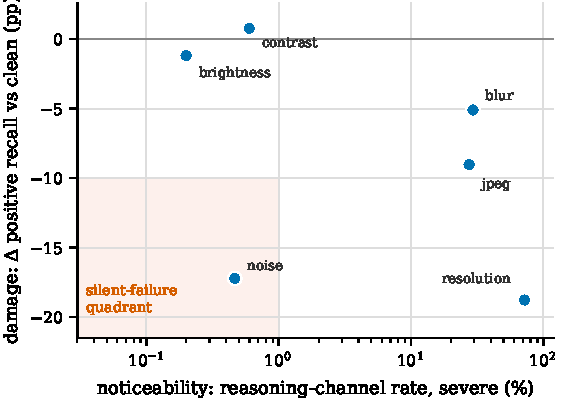
\includegraphics[width=0.62\textwidth]{figures/fig03_silent_failure.pdf}
\caption{The silent-failure quadrant (MedGemma-1.5, the only model in the matrix with a readable reasoning channel). Marker-based noticeability is the reasoning-channel rate at severe degradation; damage is the change in pooled positive recall. The shaded region is low noticeability with substantial damage; noise sits in it.}
\label{fig:silent}
\end{figure}

\subsection{The contract decides the form of the shortcut}
\label{sec:results-schema}

Holding the model, prompt content, and blank image fixed, five schemas produce two disjoint failure forms (Table~\ref{tab:schema}). Four schemas yield \textbf{0/1,506} schema-compliant blank replies, each asserting \texttt{no\_finding} positive with probability 1.0. The per-label schema with an \texttt{uncertain} state yields \textbf{1,506/1,506} compliant replies, 75\% of slots abstained and \texttt{no\_finding} positive in 0\%. The Wilson intervals do not overlap.

\begin{table}[t]
\centering
\small
\caption{Schema ablation, MedGemma-4B ($n=1{,}506$ per cell).}
\label{tab:schema}
\begin{tabular}{lrrrr}
\toprule
Schema & Blank compliance & Blank \texttt{no\_finding} pos. & Real recall & Blank abstention \\
\midrule
v0 simple & 0/1,506 & 1.000 & \textbf{0.499} & 0\% \\
v1 per-label binary & \textbf{1,506/1,506} & 0.000 & 0.442 & \textbf{75\%} \\
v2 few-shot & 0/1,506 & 1.000 & 0.269 & 0\% \\
v3 report-first & 0/1,506 & 1.000 & 0.315 (22.3\% unparsed) & 0\% \\
v4 normality pressure & 0/1,506 & 1.000 & \textbf{0.166} & 0\% \\
\bottomrule
\end{tabular}
\end{table}

The same experiment reverses the usual reading of prompt sensitivity: the schema that produces the best \emph{real-image} recall (v0) is the schema that produces the most confident \emph{blank-image} assertion. ``Prompt tuning'' and ``grounding diagnostics'' therefore cannot substitute for each other. The replication on a second medical model and the wording control are Sections~\ref{sec:results-schema2} and~\ref{sec:results-paraphrase}.

\subsection{Responsiveness collapses out of domain}
\label{sec:results-collapse}

Table~\ref{tab:audit} shows the collapse; here we test the obvious confound. PadChest has a lower disease-positive rate than NIH (17.7\% of studies carry at least one disease label vs.\ 92.0\% on NIH; the remaining NIH studies are no-finding-only), so ``always normal'' is a better prior on PadChest. Restricting to the \textbf{265 disease-positive studies}, five of six models still collapse: MedGemma-4B 8 distinct (top 90.6\%), InternVL3.5 2 (89.4\%), Qwen3-VL 2 (99.6\%), CheXagent 2 (95.5\%), Qwen2.5-VL 1 (100\%); only MedGemma-1.5 holds at 91 (34.7\%). A model that emits one answer for its disease-positive studies is not ``conservative''; it is non-responsive, and its blank contrast is unidentifiable (Figure~\ref{fig:resp}). This also explains the cross-dataset transfer result: a constant function has AUROC 0.5 by construction. The two observations are the same fact viewed twice.

\textbf{The seventh model, run on the prose layers.} LLaVA-Med was run on PadChest, Open-i, and a 200-study NIH subset rather than the full 28,614-cell grid, because the subset already shows the same constant template. It is a \emph{two-template} model: on 1,500 PadChest studies it emits 19 distinct replies, of which 59.1\% are one template, 23.3\% are empty strings, and 2.1\% are a safety disclaimer; its PadChest blank replies are 100\% empty. On Open-i it emits exactly two replies: 67.05\% ``The chest radiograph appears to be uninterpretable'' and 32.95\% a fixed normal sentence, with no finding-level content on any study. On the NIH subset it again emits two distinct replies, one covering 98.7\%, and parses as structured output on 0\% of studies; its blank replies are empty. We therefore report it as a \emph{measured} exclusion rather than a design exclusion, and do not score it on findings (Table~\ref{tab:audit}).

\begin{figure}[t]
\centering
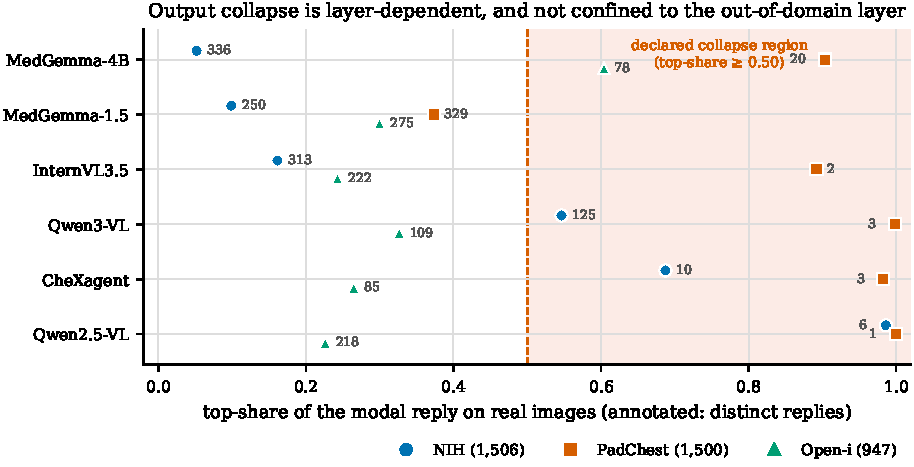
\includegraphics[width=\textwidth]{figures/fig02_responsiveness.pdf}
\caption{Responsiveness across the three layers. Each marker is the top-share of the modal reply on real images; the number beside it is the count of distinct replies. The shaded region is the pre-declared collapse rule.}
\label{fig:resp}
\end{figure}

\subsection{A blank contrast without a null is not a reliance measure}
\label{sec:results-null}

Every model's blank reply collapses to a very small set of templates---1--2 for five models, and 11 boilerplate variants for Qwen2.5-VL, of which the modal variant covers 39.7\%. For Qwen3-VL and CheXagent that template is a \textbf{refusal} (``The study is uninterpretable\ldots'', 96.3\% and 100\% of blanks); for the other four it is a \textbf{generic normal report}. In every case the correct zero is the real-vs-real similarity, not zero similarity (Table~\ref{tab:blanknull}, Figure~\ref{fig:null}).

\begin{table}[t]
\centering
\small
\caption{Open-i blank contrast against its real-vs-real null ($n=947$). $\Delta_{\text{null}} = J(\text{real},\text{real}') - J(\text{real},\text{blank})$ is the distance-based separation of Section~\ref{sec:preconditions}: positive means the blank reply is farther from the real reply than a random real reply is.}
\label{tab:blanknull}
\begin{tabular}{lrrrl}
\toprule
Model & $J(\text{real},\text{blank})$ & $J(\text{real},\text{real}')$ & $\Delta_{\text{null}}$ & Blank template \\
\midrule
CheXagent & 0.277 & 0.247 & $-0.030$ & refusal \\
Qwen3-VL & 0.091 & 0.740 & $+0.648$ & refusal \\
Qwen2.5-VL & 0.576 & 0.770 & $+0.193$ & second boilerplate \\
InternVL3.5 & 0.562 & 0.673 & $+0.112$ & generic normal \\
MedGemma-1.5 & 0.736 & 0.648 & $-0.087$ & generic normal \\
MedGemma-4B & 0.894 & 0.824 & $-0.070$ & generic normal \\
\bottomrule
\end{tabular}
\end{table}

The ranking implied by the raw Jaccard (Qwen3-VL most grounded, MedGemma-4B least) is not supported once the template is inspected. The purest case is LLaVA-Med: 67.05\% of its real Open-i replies are byte-identical to its blank refusal, and the remaining 32.95\% are one normal sentence---two templates, no findings. The PadChest collapse is not an artifact of empty strings: restricting to the 1,150 non-empty replies leaves 18 distinct strings, with the modal one covering 77.0\%. The structured layers behave the same way: all six blank replies collapse to one JSON template. The probability-space separation is the only structured statistic that separates the models, and it separates only three: MedGemma-4B ($+0.131$ NIH), InternVL3.5 ($+0.041$ NIH), MedGemma-1.5 ($+0.134$ PadChest). For every other model-layer cell the correct report is ``no measurable effect,'' not ``zero reliance.''

\begin{figure}[t]
\centering
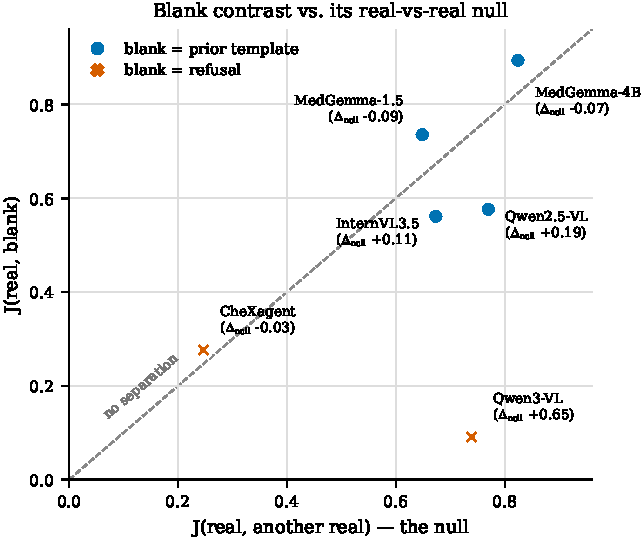
\includegraphics[width=0.62\textwidth]{figures/fig05_blank_null.pdf}
\caption{Blank contrast against its own null. Points on the diagonal have no separation; points below it are more distinct than a random real report. Refusals (crosses) are far below but measure absence detection, not evidence extraction.}
\label{fig:null}
\end{figure}

\subsection{Precision changes the output regime, not just the weights}
\label{sec:results-precision}

Table~\ref{tab:precision} (Appendix~\ref{app:protocol}) holds the model, the design, the data, and every prompt fixed; only precision changes. MedGemma-1.5 is the only model that changes regime, and its reliance ``crosses a tier'' (0.129 sits with Qwen3-VL's 0.165; 0.284 sits with MedGemma-4B's 0.296). The control model shows no regime change: its marker is 0 in both precisions and its blank answer is already \texttt{no\_finding}-positive in both; its VRS change is small and reversed (0.87$\times$). The measured dependence on precision is therefore \textbf{0.87$\times$--5.22$\times$ and not directionally universal}, but the cross-tier case is real and would corrupt any mixed-precision ranking table.

\subsection{The label-level degradation hierarchy is model-invariant on NIH}
\label{sec:results-labels}

Across four readable models on NIH, the ordering of severe-degradation recall retention by finding is concordant in the raw ranks: pairwise Spearman \textbf{0.657--0.857}, Kendall 0.619--0.786 ($n_{\text{labels}}=6$--7). Pooled retention: cardiomegaly 0.945 $>$ atelectasis 0.877 $>$ edema 0.716 $>$ consolidation 0.669 $>$ pneumonia 0.629 $>$ pneumothorax 0.605. The pneumothorax mean uses the three models with a defined ratio; Qwen3-VL has zero clean recall and its ratio is undefined, so the denominator is not fixed across labels. Two labels with near-zero clean recall (\texttt{pleural\_effusion}, \texttt{no\_finding}) produce ratios above 1 and must be excluded or reported as absolute recall.

Prevalence is a confounder, and we report it rather than let a reviewer find it. Retention correlates with NIH prevalence across labels (Spearman 0.43--0.71), and high-prevalence labels have higher mean retention in every model (Appendix~\ref{app:risk}, Table~\ref{tab:hierarchy}). After rank-residualising prevalence, pairwise partial Spearman ranges from $-0.69$ to $+0.85$ and its sign changes across pairs, so the raw concordance is not a prevalence-independent law. Per-label patient-cluster bootstrap gives 22 of 28 model--label recall changes at Benjamini--Hochberg $q<0.05$; the exceptions are cardiomegaly and the near-zero-recall pneumothorax (Appendix~\ref{app:risk}, Table~\ref{tab:perlabel}). This is \emph{model-invariance on one dataset, partly confounded by prevalence}: consistent with a lesion-level effect, but not a demonstrated dataset-invariant or prevalence-independent rule. The practical consequence is a candidate design rule---stratify robustness by finding---not a claim that finding identity alone determines degradation sensitivity. External replication is needed before treating it as transferable.

\subsection{Cross-dataset discrimination collapses}
\label{sec:results-transfer}

\begin{table}[t]
\centering
\small
\caption{AUROC on NIH vs.\ PadChest for representative labels. 95\% intervals are patient-cluster bootstrap over the target domain.}
\label{tab:transfer}
\begin{tabular}{lrrr}
\toprule
Model & \texttt{no\_finding} NIH $\rightarrow$ PadChest & \texttt{cardiomegaly} NIH $\rightarrow$ PadChest & $\Delta$ CI (cardiomegaly) \\
\midrule
InternVL3.5 & 0.774 $\rightarrow$ \textbf{0.500} & 0.672 $\rightarrow$ \textbf{0.500} & $[-0.201,-0.141]$ \\
Qwen3-VL & 0.685 $\rightarrow$ \textbf{0.501} & 0.598 $\rightarrow$ \textbf{0.500} & $[-0.122,-0.071]$ \\
MedGemma-4B & 0.524 $\rightarrow$ 0.508 & 0.690 $\rightarrow$ \textbf{0.492} & $[-0.236,-0.154]$ \\
MedGemma-1.5 & 0.499 $\rightarrow$ 0.496 & 0.675 $\rightarrow$ \textbf{0.541} & $[-0.200,-0.061]$ \\
Qwen2.5-VL & 0.508 $\rightarrow$ 0.500 & 0.504 $\rightarrow$ 0.500 & $[-0.011,+0.002]$ \\
CheXagent & 0.504 $\rightarrow$ 0.500 & undefined (constant; 87 positives) & --- \\
\bottomrule
\end{tabular}
\end{table}

Only MedGemma-1.5 retains a cardiomegaly AUROC above chance (0.541, interval excludes 0.5), and it is also the only model that holds its responsiveness (Table~\ref{tab:transfer}). The two facts are consistent: a model that produces one answer cannot rank images, and a model that ranks images must produce more than one answer (Figure~\ref{fig:transfer}). The collapse is not VLM-specific: the same DenseNet-121 reaches only 0.515 macro AUROC on PadChest against 0.733 on NIH (Appendix~\ref{app:risk}, Table~\ref{tab:densenetgrid}), so a supervised model trained on one hospital also fails to transfer.

The comparison changes hospital source, case mix, label mapping, and input geometry together, so the drop is a \emph{cross-dataset} effect, not an isolated hospital effect. The common-label recomputation (Appendix~\ref{app:risk}) removes the structurally missing pneumonia term, and the responsiveness check removes the constant-output explanation, but no design here separates hospital shift from case-mix shift. We therefore claim dataset-level discrimination collapse, not a quantified hospital-domain penalty. At the label level the hierarchy is not estimable out of domain: the five non-responsive models emit at most 20 distinct replies and their per-label AUROC sits at 0.492--0.536 without a meaningful ranking, while for the one responsive model (MedGemma-1.5) only cardiomegaly has an interval above chance (0.541, 95\% CI 0.505--0.584; atelectasis 0.531, CI 0.464--0.605) and the remaining four estimable labels sit at 0.489--0.490 (Appendix~\ref{app:risk}, Table~\ref{tab:padlabel}). The NIH label ordering does not transfer as a rankable hierarchy; what transfers is the collapse itself.

\begin{figure}[t]
\centering
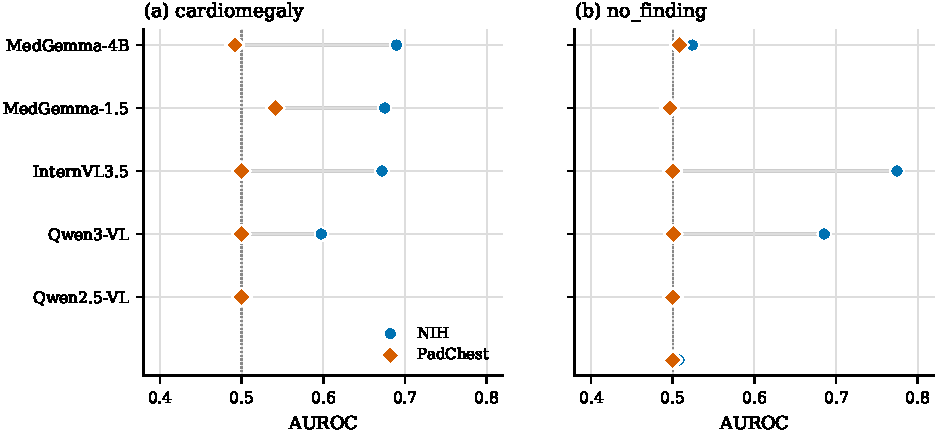
\includegraphics[width=\textwidth]{figures/fig04_transfer.pdf}
\caption{Cross-dataset transfer (NIH $\rightarrow$ PadChest). Each segment connects the NIH AUROC to the PadChest AUROC for the same model; the dotted line is chance.}
\label{fig:transfer}
\end{figure}

\subsection{The report layer: a labeller-dependent ordering}
\label{sec:results-report}

The full Open-i table is Appendix~\ref{app:protocol}, Table~\ref{tab:report}. The ordering is labeller-dependent. Under the rule-based labeller the two error types order the six models in opposite directions; under CheXbert, applied to the same 947 studies, the hallucination ordering is preserved in direction (Spearman 0.71, $n=6$, $p=0.11$) but the omission ordering is not ($-0.49$, $p=0.33$; Appendix~\ref{app:protocol}, Table~\ref{tab:chexbert}). We therefore do not claim a universal omission--hallucination trade-off: the apparent trade-off is a property of the rule-based labeller, and only the hallucination axis is stable enough to report as a model ordering.

\subsection{Selective prediction: no usable coverage}
\label{sec:results-selective}

Selective metrics require a schema adapter: the matrix runners nest the answer under \texttt{parsed.findings} and the NIH reliance file carries no ground truth, so pointing the existing selective-prediction scripts directly at them yields zero rows. This subsection is also the downstream cost of the four preconditions: a selective-trust layer can be no more identifiable than the contract it consumes, and its coverage is bounded by contract coverage before any risk model is fitted. With the adapter, the compliance coverage differs sharply across models: Qwen2.5-VL 100\%, InternVL3.5 99.6\%, MedGemma-1.5 95.2\%, Qwen3-VL 91.7\%, MedGemma-4B 87.9\%, \textbf{CheXagent 18.9\%}. The per-cell coverage census is in Appendix~\ref{app:protocol}, Table~\ref{tab:coverage}.

CheXagent therefore produces two mutually inconsistent image-level error rates depending on the convention: 0.183 when labels without a probability are skipped, 1.000 when every non-positive status is treated as negative. Neither is wrong; they answer different questions. Its selective metrics are not comparable with the other five and are reported with \texttt{contract\_coverage} $=0.189$ (\texttt{not\_mentioned} $=9{,}486/12{,}016$ slots; only 9.7\% of images have all eight definite).

\begin{table}[t]
\centering
\footnotesize
\caption{Selective prediction on the held-out NIH test split ($n=1{,}054$ studies; 8,432 finding items; 427 patient clusters). ``Risk'' is the error rate among answered items. AUROC columns are finding-level error-detection AUROC for confidence alone and for confidence plus the shift score.}
\label{tab:selective}
\begin{tabular}{lrrrrrrr}
\toprule
Model & Finding error & Cov.\ @5\% & Cov.\ @10\% & Risk @50\% cov. & Risk @80\% cov. & AUROC (conf.) & $+$ shift \\
\midrule
MedGemma-4B & 0.335 & 0.064 & 0.249 & 0.232 & 0.322 & 0.644 & 0.678 \\
MedGemma-1.5 & 0.323 & 0.093 & 0.332 & 0.173 & 0.270 & 0.737 & 0.737 \\
InternVL3.5 & 0.319 & 0.000 & 0.117 & 0.235 & 0.302 & 0.627 & 0.635 \\
Qwen3-VL & 0.392 & 0.010 & 0.025 & 0.256 & 0.377 & 0.660 & 0.664 \\
Qwen2.5-VL & 0.440 & 0.005 & 0.020 & 0.234 & 0.375 & 0.772 & 0.773 \\
\bottomrule
\end{tabular}
\end{table}

Image-level error is ceiling-dominated: every NIH evaluation study is positive for at least one of the eight labels (92\% for at least one disease; the remainder are no-finding-only), so an all-negative predictor scores 0 and 0.94--0.97 is an upper-bound artifact of composition. The finding level is the interpretable one (Table~\ref{tab:selective}). At that level, adding the shift score to confidence changes AUROC by at most $+0.034$ (MedGemma-4B 0.644$\rightarrow$0.678, InternVL3.5 0.627$\rightarrow$0.635, Qwen3-VL 0.660$\rightarrow$0.664, Qwen2.5-VL 0.772$\rightarrow$0.773) and does not move MedGemma-1.5 (0.737$\rightarrow$0.737); adding image reliance moves the two MedGemma models by $+0.033$ and $+0.006$. Ranking is therefore close to what confidence alone already provides, while no model exceeds 9.3\% coverage at a 5\% risk budget. The three-action policy never accepts at the image level (accept rate 0.000). At the finding level it accepts 17--41\% of items for the five comparable models (CheXagent 12--17\% under its 18.9\% contract), but the accepted error rate is 5.7--21.7\%, above the 5\% budget in every cell. It therefore fails the budget at the only level where it can act, rather than by refusing to act.

The full risk--coverage curves (Appendix~\ref{app:risk}, Figure~\ref{fig:risk}) show why the 5\% negative result is not an artifact of one threshold. At 5\% coverage the risk is already 0.043--0.154, and by 10\% coverage every model exceeds the 5\% budget. Coverage at a 10\% budget is 0.020--0.332, and risk at 50\% and 80\% coverage is 0.173--0.256 and 0.270--0.377 respectively. The policy never reaches a usable operating point at 5\%; whether it does at a clinically sanctioned 10--20\% budget is a decision for a deployment, not a claim of this paper.

\subsection{Controlled replications}
\label{sec:results-round2}

The 2026 literature left three questions that decide how much of the above travels: whether a supervised model would also sit at chance, whether the schema result is one checkpoint's habit, and whether a second reasoning model shows the same axes. This section answers the three with pre-deployed controls rather than post-hoc argument, and tests the fourth---cross-family generality---for the schema result; the remaining cross-family claims are still open and flagged as such.

\subsubsection{A supervised baseline is not at chance}
\label{sec:results-baseline}

We trained DenseNet-121~\citep{huang2017densely} from ImageNet initialisation at $224$\,px with a class-weighted BCE objective, AdamW, and a fixed eight epochs with no early stopping or test-time model selection. It saw only the 3,871 \texttt{internal\_train} images and shares no patient with the 1,506 evaluation studies (patient overlap 0). On the same seven pathology labels it reaches \textbf{macro AUROC 0.733} (95\% patient-cluster bootstrap CI 0.718--0.749, 725 patients, 1,000 resamples; per-label 0.620--0.805; Table~\ref{tab:baseline}), and 0.724 on its own patient-disjoint 1,352-study \texttt{internal\_test} split (the VLM evaluation uses the 1,054-study subset of that split; Section~\ref{sec:protocol}).

\begin{table}[t]
\centering
\small
\caption{Clean NIH macro AUROC over the seven pathology labels, $n=1{,}506$. The baseline trains on 3,871 disjoint-patient images only; the six VLMs are the matrix from Table~\ref{tab:clean}.}
\label{tab:baseline}
\begin{tabular}{lrr}
\toprule
Model & Macro AUROC & Family \\
\midrule
\textbf{DenseNet-121 (supervised)} & \textbf{0.7329} & CNN, trained here \\
MedGemma-4B & 0.6270 & medical VLM \\
InternVL3.5-8B & 0.6066 & general VLM \\
MedGemma-1.5 & 0.5852 & medical VLM \\
Qwen3-VL-8B & 0.5455 & general VLM \\
Qwen2.5-VL-7B & 0.5013 & general VLM \\
CheXagent-8B & 0.5001 & CXR specialist \\
\bottomrule
\end{tabular}
\end{table}

The labels are therefore learnable from these images at $0.73$, from 3,871 training images---under 5\% of the 86{,}524-image released training split. ``No usable discrimination'' is a statement about the models, not about the task or the label noise alone. The baseline also bounds the claim in the other direction: 0.73 is not clinical-grade, so the paper's negative result concerns \emph{measurement identifiability} at this performance level, not the impossibility of CXR classification.

\subsubsection{Schema dependence replicates on a second medical model, with a different mapping}
\label{sec:results-schema2}

We repeated the five-schema sweep on MedGemma-1.5 (15,060 calls). The headline result replicates: on a blank image, \textbf{all five schemas produce pathology recall 0.000}, against 0.493--0.614 on real images (Table~\ref{tab:r2schema}). No wording creates image dependence.

What does \emph{not} replicate is which failure form each schema takes. MedGemma-4B had two forms (confident normal, or forced abstention). MedGemma-1.5 shows three: confident normal (\texttt{no\_finding} positive in 100\% of blank replies for v0, v1 and v3), a \emph{contract collapse} (v2 returns labels but drops the probability object in 99.9\% of blank replies), and refusal to assert (v4 returns \texttt{no\_finding} negative in 100\% of blank replies with the same contract collapse). The schema with the highest real-image recall is v4 (0.614, $+6.3$\,\pp{} over v0) while its blank recall stays 0.000: the prompt moved the operating point, not the model's access to evidence.

The correct reading is therefore narrower than ``the contract decides the form of the shortcut'' (Section~\ref{sec:results-schema}): the contract and the model \emph{jointly} decide it, and the joint mapping is not transferable across checkpoints. What transfers is the invariance that matters for a benchmark: real-image recall and blank-image behaviour are set by different things, so a schema cannot be validated on either alone.

\subsubsection{The blank-image result travels across a model family; the contract signature does not}
\label{sec:results-xfamily}

To separate a MedGemma habit from a contract effect we repeated the sweep on Qwen3-VL-8B, a general model from a different family (Table~\ref{tab:r2xfamily}). The blank-image result replicates exactly: pathology recall is \textbf{0.000} on the blank image under all three schemas, against 0.258--0.306 on real images. The observable signature does not replicate. Qwen3's v0 is confident-normal (\texttt{no\_finding} positive in 100\% of blank replies) but emits only one of the eight requested probabilities, so probability completeness is 12.5\% on blank and 47.1\% on real; v1 keeps the same confident-normal answer while restoring completeness to 100\% and 95.2\%; v4 refuses the normal assertion (\texttt{no\_finding} positive in 0\% of blanks) and collapses the contract in 98\% of real replies. The same three-form structure appears in both models, with a different variant-to-form mapping. Contract coverage is therefore a property of the schema, not of the model, while the blank-image dependence is a property of both.

\begin{table}[t]
\centering
\footnotesize
\setlength{\tabcolsep}{3.5pt}
\caption{Cross-family schema sweep on Qwen3-VL-8B ($n=1{,}506$ per cell). Blank-image pathology recall is 0.000 under all three schemas, so the blank dependence is not a MedGemma habit. The observable signature differs: v0 is confident-normal with one probability emitted, v1 is confident-normal with a complete contract, v4 refuses the normal assertion and collapses the contract.}
\label{tab:r2xfamily}
\begin{tabular}{lrrrrrr}
\toprule
Variant & Real recall & Blank recall & Blank \texttt{no\_finding} pos. & Violation (real/blank) & Completeness (real/blank) \\
\midrule
v0 simple & 0.306 & \textbf{0.000} & 1.000 & 0.611 / 1.000 & 0.471 / 0.125 \\
v1 per-label binary & 0.258 & \textbf{0.000} & 1.000 & 0.054 / 0.000 & 0.952 / 1.000 \\
v4 normality pressure & 0.263 & \textbf{0.000} & 0.000 & 0.983 / 1.000 & 0.849 / 0.875 \\
\bottomrule
\end{tabular}
\end{table}

\subsubsection{Wording is not the mechanism, but it sets the blank-image answer}
\label{sec:results-paraphrase}

Two paraphrases of the v0 contract, identical in label set, status rule and JSON shape, were run against real and blank images on MedGemma-4B (6,024 calls). On real images the finding-level answer is reproducible: 90.9\% and 91.4\% agreement with the v0 baseline, Cohen's $\kappa$ 0.624 and 0.642. The schema result is not a single-wording artifact.

On blank images the same two paraphrases disagree with the baseline on exactly one label. v0 asserts \texttt{no\_finding} positive in 100\% of blank replies; p2 does the same (agreement 1.000); p1 asserts it negative in 100\% (agreement 0.000). Pathology labels are identical across all three (all negative, agreement 1.000). A blank image therefore yields an answer that is a function of the wording and carries no image information---which is precisely why the null-model precondition needs a blank control \emph{and} a wording control, not either alone.

The control also runs on Qwen3-VL (Table~\ref{tab:r2para}). Both paraphrases reproduce the real-image answer (p1 93.1\% agreement, $\kappa$ 0.723; p2 90.3\%, $\kappa$ 0.701), but neither flips the blank-image answer: agreement with v0 on the blank image is 1.000 for both, whereas p1 flips MedGemma-4B's blank answer completely. Wording therefore sets a prior that is model-specific: the same paraphrase that turns MedGemma's blank answer negative leaves Qwen3's confident-normal answer intact.

\subsubsection{A second reasoning model: same operating point, new failure mode}
\label{sec:results-second}

Qwen3-VL-8B-Thinking exposes a native reasoning channel (the chat template pre-fills \texttt{<think>}, the model closes it before answering), so the noticeability axis is readable in a second model for the first time. We ran seven cells (clean plus six severe) on all 1,506 studies. A reply counts only if it closes the reasoning block \emph{and} a JSON object parses after the close; the rest are retained as a measured outcome (Table~\ref{tab:r2recon}).

\textbf{Coverage is a measurable quantity, and it degrades with damage.} At a 5,120-token budget the model produces a usable answer on 9,381 of 10,542 cells (89.0\%); the 8,192-token sample of 40 cells adds 20 (89.2\% final). Coverage is 92.6\% on clean images, 80.9\% on resolution-severe, 84.3\% on brightness-severe (Table~\ref{tab:r2think}). The failures are not truncation artefacts that a larger budget removes: replies that still fail have a median length of 9.8\,k characters at a 2,560-token cap, 13.5\,k at 3,584, 19.3\,k at 5,120, and 28.1\,k in the 40-cell sample at 8,192, i.e.\ they expand to fill whatever budget they are given; that sample rescues 50\% (Table~\ref{tab:r2budget}). Non-termination is a behaviour of the model, and we report it as one. This is the vision-language counterpart of the overthinking literature: beyond some point additional reasoning tokens have negative marginal value and can abandon answers the model already had~\citep{wu2026whenmore,zhou2026overthinking}, and truncated traces can be worse than none~\citep{su2026broken}. Here the failure is more severe---the reply never becomes parsable---so the budget curve is a measurement property of the model, not only a cost.

\begin{table}[t]
\centering
\small
\caption{Second reasoning model, severe cells ($n=1{,}506$ studies per cell). Coverage is the share of studies with a usable answer at a 5,120-token budget; $\Delta$ recall is paired against clean on studies answered in both cells (noise $n=1{,}238$; resolution $n=1{,}132$). AUROC is macro over the seven pathology labels; positive rate is the share of pathology slots called positive.}
\label{tab:r2think}
\begin{tabular}{lrrrrr}
\toprule
Cell & Coverage & Trace (k chars) & Pos.\ rate & Macro AUROC & $\Delta$ recall \\
\midrule
clean & 0.926 & 8.73 & 0.250 & 0.547 & --- \\
blur & 0.932 & 8.84 & 0.189 & 0.547 & $-5.5$\,\pp{} \\
brightness & 0.843 & 9.56 & 0.213 & 0.550 & $-5.1$\,\pp{} \\
contrast & 0.924 & 8.99 & 0.280 & 0.545 & $+2.2$\,\pp{} \\
JPEG & 0.923 & 9.37 & 0.240 & 0.537 & $-1.8$\,\pp{} \\
noise & 0.885 & 9.06 & 0.173 & 0.527 & $\mathbf{-10.3}$\,\pp{} \\
resolution & \textbf{0.809} & \textbf{10.22} & \textbf{0.125} & 0.549 & $\mathbf{-13.2}$\,\pp{} \\
\bottomrule
\end{tabular}
\end{table}

\textbf{The operating-point mechanism replicates, in the opposite direction.} The positive-call rate falls from 0.250 to 0.125 under resolution loss, the \texttt{no\_finding} rate rises from 0.283 to 0.450, and macro AUROC is flat at 0.527--0.550 in every cell. Because coverage also falls, we recomputed the rate on the paired subset (studies answered in both cells): 0.250 $\rightarrow$ 0.128, i.e.\ the move is not a coverage artefact (Appendix~\ref{app:round2}, Table~\ref{tab:r2posrate}). The model does not lose ranking information---it never had any---it moves its operating point toward ``normal.'' This is the mirror image of Section~\ref{sec:results-op}: there, models with a high clean positive rate moved it up under damage and recall rose; here a model with a 25\% positive rate moves it down and recall falls. Both are operating-point shifts, and neither is a robustness change.

Per-label, the paired loss survives cluster bootstrap and multiplicity control: pleural effusion $-8.8$ $[-11.9,-5.8]$\,\pp{} and pneumonia $-11.0$ $[-16.4,-5.5]$\,\pp{} ($q<0.001$), cardiomegaly $-6.0$ $[-9.9,-1.9]$\,\pp{} ($q=0.014$), atelectasis $-2.2$ and edema $-4.2$\,\pp{} ($q=0.053$), consolidation and pneumothorax not significant (Table~\ref{tab:r2label}).

\textbf{The axis pair generalises; the quadrant does not.} Using coverage loss as the noticeability readout of this model and paired recall change as damage, the two quantities are again separable (Spearman 0.49 with $|\Delta|$, $p=0.33$; $-0.54$ with signed $\Delta$, $p=0.27$; $n=6$). The MedGemma-1.5 marker--damage correlation is 0.49 under the same $|\Delta|$ definition, but with six points neither estimate is distinguishable from zero: we claim the same \emph{direction}, not a common slope. Noise moves: for MedGemma-1.5 it was the silent corruption (marker 0.46\%, second-lowest) with damage comparable to resolution loss, whereas for Qwen3-VL-Thinking noise is loud (11.5\% coverage loss, third-highest) and damages recall by 10.3\,\pp{}. \emph{Silent failure is a property of the monitoring channel, not of the corruption}: a channel that watches reasoning termination sees noise, one that watches a specific marker token does not.

This also explains why the second model does not reproduce Reversal~3's positive sign. The reversal needs headroom in the positive rate; a model that calls 25\% of slots positive has little, and degradation moves it down rather than up. Reporting the operating point, as required by the fourth precondition, is what makes the two models comparable at all.


\subsection{Sensitivity of the headline judgments}
\label{sec:sensitivity}

Three of the most load-bearing thresholds were swept over their full range (Appendix~\ref{app:risk}, scripts/\url{81_sensitivity_analyses.py}). The 19-cell grid itself is an exploratory dose--response design: its per-cell contrasts are descriptive and are not multiplicity-adjusted across cells, and no family-wise claim is attached to them. The confirmatory quantities are the four audit statistics declared in Section~\ref{sec:preconditions} and the replications of Section~\ref{sec:results-round2}.

\textbf{(i) The collapse rule.} Varying the top-share threshold over $0.30$--$0.80$ and the unique-count bound over $1$--$20$ changes which marginal cells are flagged (Table~\ref{tab:sweep}), but not the cross-dataset conclusion: on PadChest five of six models are collapsed at every threshold from $0.40$ to $0.80$, and at the most permissive $0.30$ cut MedGemma-1.5---which emits 329 distinct replies---is flagged as well, so all six collapse. In-domain the flagged set narrows as the threshold rises (Qwen3-VL leaves at $0.60$, CheXagent at $0.70$); on Open-i MedGemma-4B is flagged below $0.70$, and at $0.30$ Qwen3-VL is flagged too. None of the paper's claims rests on these marginal cells.

\textbf{(ii) The real-vs-real null pairing.} For Open-i, the real-vs-real Jaccard is recomputed under (a) random image pairs and (b) reference-report-length-matched pairs. The null changes by at most $0.020$ (Table~\ref{tab:sens}; MedGemma-4B: 0.824 vs.\ 0.844), and every separation keeps its sign and magnitude: Qwen3-VL stays far above its null ($+0.648$ vs.\ $+0.643$), Qwen2.5-VL stays $+0.19$, MedGemma-4B and MedGemma-1.5 stay negative ($-0.070$ and $-0.087$). The ``the blank is a different template, not evidence'' reading is robust to the pairing rule.

\textbf{(iii) Transfer intervals under a multiplicity correction.} The cross-dataset $\Delta$AUROC intervals reported in Table~\ref{tab:transfer} are single-pairwise 95\% intervals. We recompute all 16 estimable model--label cells under a Bonferroni correction for that family ($z=2.955$). All four large losses survive: InternVL3.5 \texttt{cardiomegaly} (corrected upper bound $-0.127$), InternVL3.5 \texttt{consolidation} ($-0.048$), MedGemma-4B \texttt{cardiomegaly} ($-0.136$), and MedGemma-1.5 \texttt{cardiomegaly} ($-0.030$) remain strictly below zero. Two borderline deltas (MedGemma-4B and MedGemma-1.5 \texttt{no\_finding}) become non-significant, as do the small consolidation and cardiomegaly cells that were already near chance; the four large losses are unaffected. The claim ``transfer collapses'' is robust; a few near-zero cells are not.

\textbf{(iv) Operating-point composition.} The InternVL3.5 contrast/severe cell decomposes at the level of individual images (Appendix~\ref{app:risk}). Across the three findings with the most transitions, the ``recall gain'' is entirely new true positives on images that were negative under the clean condition ($gt\_pos$: $+43$, $+30$, $+50$ gained vs.\ $10$, $3$, $1$ lost), while previously-correct negative statuses flip to false positives at a comparable rate ($gt\_neg$: $+36$, $+59$, $+69$). Net false positives rise (Table~\ref{tab:op}). This is consistent with a broad operating-point move, not a targeted recovery of lost findings; it does not by itself identify the threshold mechanism.

\begin{figure}[t]
\centering
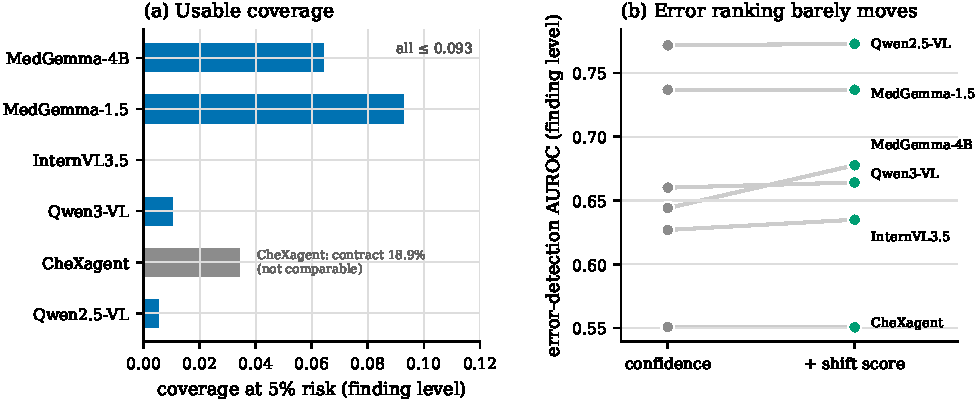
\includegraphics[width=\textwidth]{figures/fig06_selective.pdf}
\caption{(a) Usable coverage at a 5\% risk budget is at most 0.093; CheXagent's bar is grey because its contract covers only 18.9\% of slots. (b) At the finding level the same signals change error ranking only marginally. Ranking and decision usefulness are separate quantities.}
\label{fig:selective}
\end{figure}

\begin{figure}[t]
\centering
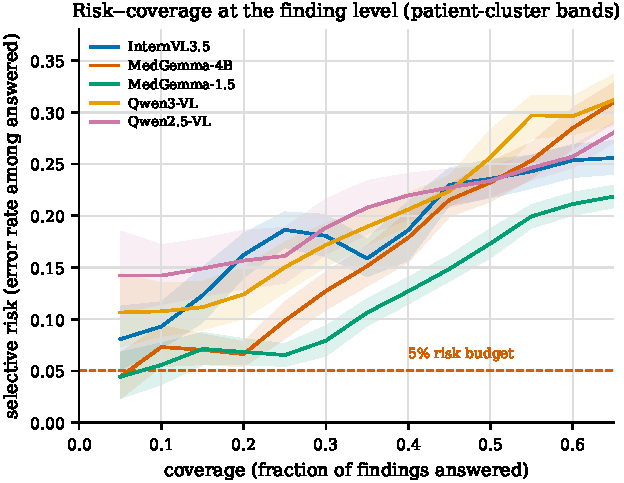
\includegraphics[width=0.62\textwidth]{figures/fig07_risk_coverage.pdf}
\caption{Risk--coverage at the finding level, with patient-cluster bootstrap bands (1,000 resamples). At 5\% coverage the risk is 0.043--0.154, and by 10\% coverage every model exceeds the 5\% budget; a 5\% budget admits at most 0.093 coverage, while a 10\% budget admits 0.02--0.33 depending on the model.}
\label{fig:risk}
\end{figure}
